\section{User Study}
We conduct a user study to evaluate the feasibility and effectiveness of our approach in facilitating coordination strategy design for agent collaboration. Our evaluation focuses on (1) The effectiveness of the structured coordination strategy generation approach. (2) The overall effectiveness and usability of the interactive system. (3) the support for coordination strategy design compared with two baseline systems based on existing LLM-based multi-agent coordination frameworks.

\subsection{Methodology}

\subsubsection{Participants}
We recruited 12 participants (P1-P12) with a general interest in LLM-based multi-agent collaboration for our experiment, 3 females and 9 males, aged 23-28 from the local university. To mitigate evaluation bias, all participants had not been involved in our formative study or the approach design process. All of the participants have ever used ChatGPT in the past. Seven have heard about at least one LLM-based multi-agent system or framework. Four have first-hand touch with at least one LLM-based multi-agent system or framework.
% All experiments were conducted offline, and participants could receive approximately \$14 upon completion.

\subsubsection{Experiment Setup}
We set up two additional baseline systems for comparative study \cite{wong2023anchorage, feng2023promptmagician, feng2023xnli} alongside our system. All three systems utilize GPT4 as the default LLM model. The users can also use ChatGPT at their will during experiments. During the strategy design phase in \textit{AgentCoord}, we allow users to switch to a fast mode that uses Mistral 8$\times$7B model with hardware acceleration\footnote[5]{{https://groq.com/}} for the first time of generation to strike a balance of response quality and efficiency. The agents used in the experiments are generated through role prompting \cite{Expertprompting} and then converted to the corresponding format required for the three systems.


\textbf{Baseline A} (AutoAgents with simple UI): provides a set of carefully designed prompts to let the LLM generate a step-by-step coordination strategy for collaboration based on the goal provided by the user. Each step starts with a list ``[name1, name2, ..]'' to specify the agents involved and uses natural language to specify how agents will collaborate. A simple text editor is provided for further editing the strategy. Once the user is satisfied, they can click the ``execute'' button to start collaboration. The output of the execution result is shown in the text terminal.

\textbf{Baseline B} (AutoGen in Group Chat Mode): allows adding multiple LLM-based agents in a group chat and coordinating them using natural language. During the coordination strategy design, a planner agent first drafts an initial coordination strategy based on the general goal provided by the user and the profile of available agents. The user plays the role of an admin agent and refines the coordination strategy collaboratively with the planner agent by chatting. Once the user is satisfied with the coordination strategy, they can start the collaboration. The output of the execution result is shown in the text terminal.

\subsubsection{Procedure}
\textbf{Introduction and Training}: We initially briefed the users on the objective and relevant context of the experiment. Following that, we gathered basic information from the users, along with their exposure to LLM-based multi-agent systems or frameworks. Afterward, we demonstrated to the participants how to design coordination strategies for agents using the three systems. We allowed the participants adequate time to experiment with and familiarize themselves with the systems. During this process, they were free to ask questions at any point. 

\textbf{Task Process}: For each system, participants are required to select a general goal (e.g. ``\textit{write an engaging tutorial about bubble sort for kids}'', ``\textit{make a content strategy for a local weekend event}'') for agent collaboration and design coordination strategy for it with the given system. During the design process, the participants are required to finish four sub-tasks: 1. Comprehend and judge the coordination strategy generated by the system. 2. Explore and improve at least three different aspects of the generated collaborative strategy. 3. Execute the collaborative strategy at least once and analyze the results. 4. Improve at least one area of the original collaborative strategy based on the execution results. After the user meets the requirements for the sub-tasks, they can continue open-ended exploration with the system freely without time constraints. The order of the systems was counterbalanced.

\textbf{Semi-structured interview}: 
We ask participants to fill out a five-point Likert-scale questionnaire designed to assess our system's effectiveness and usability (\cref{fig:effectiveness and usability}), and coordination support comparison for all systems (\cref{fig:Coordination Support Comparison}). For each question, we encourage participants to explain the reasoning for their ratings and provide any opinion. In the end, we collect overall feedback about our system from users.

\subsection{Results Analysis}


\subsubsection{Effectiveness of Structured Strategy Generation}
Most of the participants agreed that the structure for coordination strategy is expressive and easy to understand (Q1). Users praised that the structure is ``\textit{clear}'' (P5) and ``\textit{intuitive}'' (P2). P5 commented, ``\textit{it goes from high level to low level, which makes sense. The connections between each part are really clear.}'' P7 told us that ``\textit{the proposed classification for interaction type is very helpful}'' and ``\textit{hope the later versions of the system support customizing and managing different levels of classification granularity}''. Most of the participants agreed that the structure for coordination strategy facilitates the design process (Q2). The users appreciated the structure ``\textit{provide a clear map for what have been explored and what could be explored next}'' (P11) and ``\textit{make the exploration process more systematic and confident}'' (P8). P10 told us that ``the structure helps increase the predictability and my confidence when prompting LLM during exploration''. Most of the participants agree that the generated initial strategy is helpful as a starting strategy (Q3). The users found the baseline strategy always at least serves a ``\textit{fair starting point}'' (P6) and sometimes ``\textit{unexpectedly good}'' (P3). Some users express the demand to ``\textit{have someplace to enter user's preference or prior knowledge to affect the starting generation}'' (P5).



\subsubsection{Effectiveness of Interactive System}

\textbf{Visual Organization for Strategy.} Most of the participants agreed that the visual organization for coordination strategy facilitates comprehension (Q4). The \textit{Plan Outline View} is regarded helpful for ``\textit{quickly get an understanding of the overall strategy}'' (P2) and ``\textit{convenient for navigation}'' (P9). P11 commented, ``\textit{I like the `parallel line design', the relationship between tasks is clearly illustrated}''. Users appreciated ``the adaptive informative reviling'' (P6) in \textit{Agent Board View} while wishing for allowing to ``\textit{show an agent’s historical performance on need}'' (P5). The text highlighting in \textit{Task Process View} is widely praised by users for aiding fast comprehension. However, some users still found the quantity of text to read for task process specification is large and wish to ``\textit{have a summary for each action instruction}'' (P3). The overall layout is also praised by some users in terms of aesthetics and consistency. 

\textbf{Interactive Exploration for Alternative Strategy.} Users generally appreciate the exploration interactions supported by our system. Meanwhile, users find the organization for exploration histories to be `extremely convenient' (P7) and `helpful in focusing on exploration' (P10). Nevertheless, we noted variations in how often and how favorably users engaged with the three exploration views (Q5,6,7). While both the \textit{Plan Outline Exploration View} and the \textit{Process Exploration View} are for sequential structure exploration and share a similar design, we find generally participants tend to do more exploration in the \textit{Plan Outline Exploration View}. P5 explained: ``\textit{when deciding the outline for the overall collaboration, I am not sure how to do and want to see more possibilities, branching with high-level natural language requirement is extremely useful at that phase. On the other hand, the task process is for a more detailed level, which I usually do not want to spend too much time exploring and just want to directly modify}'' (P5). The \textit{Agent Assignment Exploration View} is the most popular view for exploration. Most users find using head-map to visualize LLM's prior knowledge for agent assignment ``\textit{is comprehensive and insightful}'' (P4) and the interactions ``\textit{flexible and engaging for exploration}'' (P10). 


\textbf{Execution Result Examination.} Most of the participants agreed that the \textit{Execution Result View} facilitates the analysis of the execution result (Q8). The participants confirmed that when examining the result, it is easy to connect any part of the result with its corresponding strategy design. P7 commented: ``\textit{when I want to a analyze certain result, I just click it, the other views automatically show relevant strategy information, reminding me of my previous design process, that's cool.}'' The trace lines for important action inputs were also found helpful. P9 mentioned that he likes starting with the final result of a certain task and leveraging the trace lines to help trace back to see how this final result is formed along the way to identify possible points for improvement.

\subsubsection{Usability}
Most of the participants agreed that our system was easy to learn (Q9)
and easy to use (Q10). Participants commented that the interface of
our system was ``\textit{intuitive}'' (P2) and ``\textit{clear}'' (P5). Several users reported although each feature of the system is each to understand, it still requires some time to fully master the system in order to use it fluently. All of the participants express their willingness to use our system again (Q11). P5 told us that he wish to ``\textit{use this system to coordinate some agents to help maintain my blog in the future}'' (P5). P1 expressed the willingness to use our system to fast prototype some coordination strategies for research purposes, indicating its potential to contribute to the research community for LLM-based multi-agent systems.

\begin{figure}[!t]
    \centering
    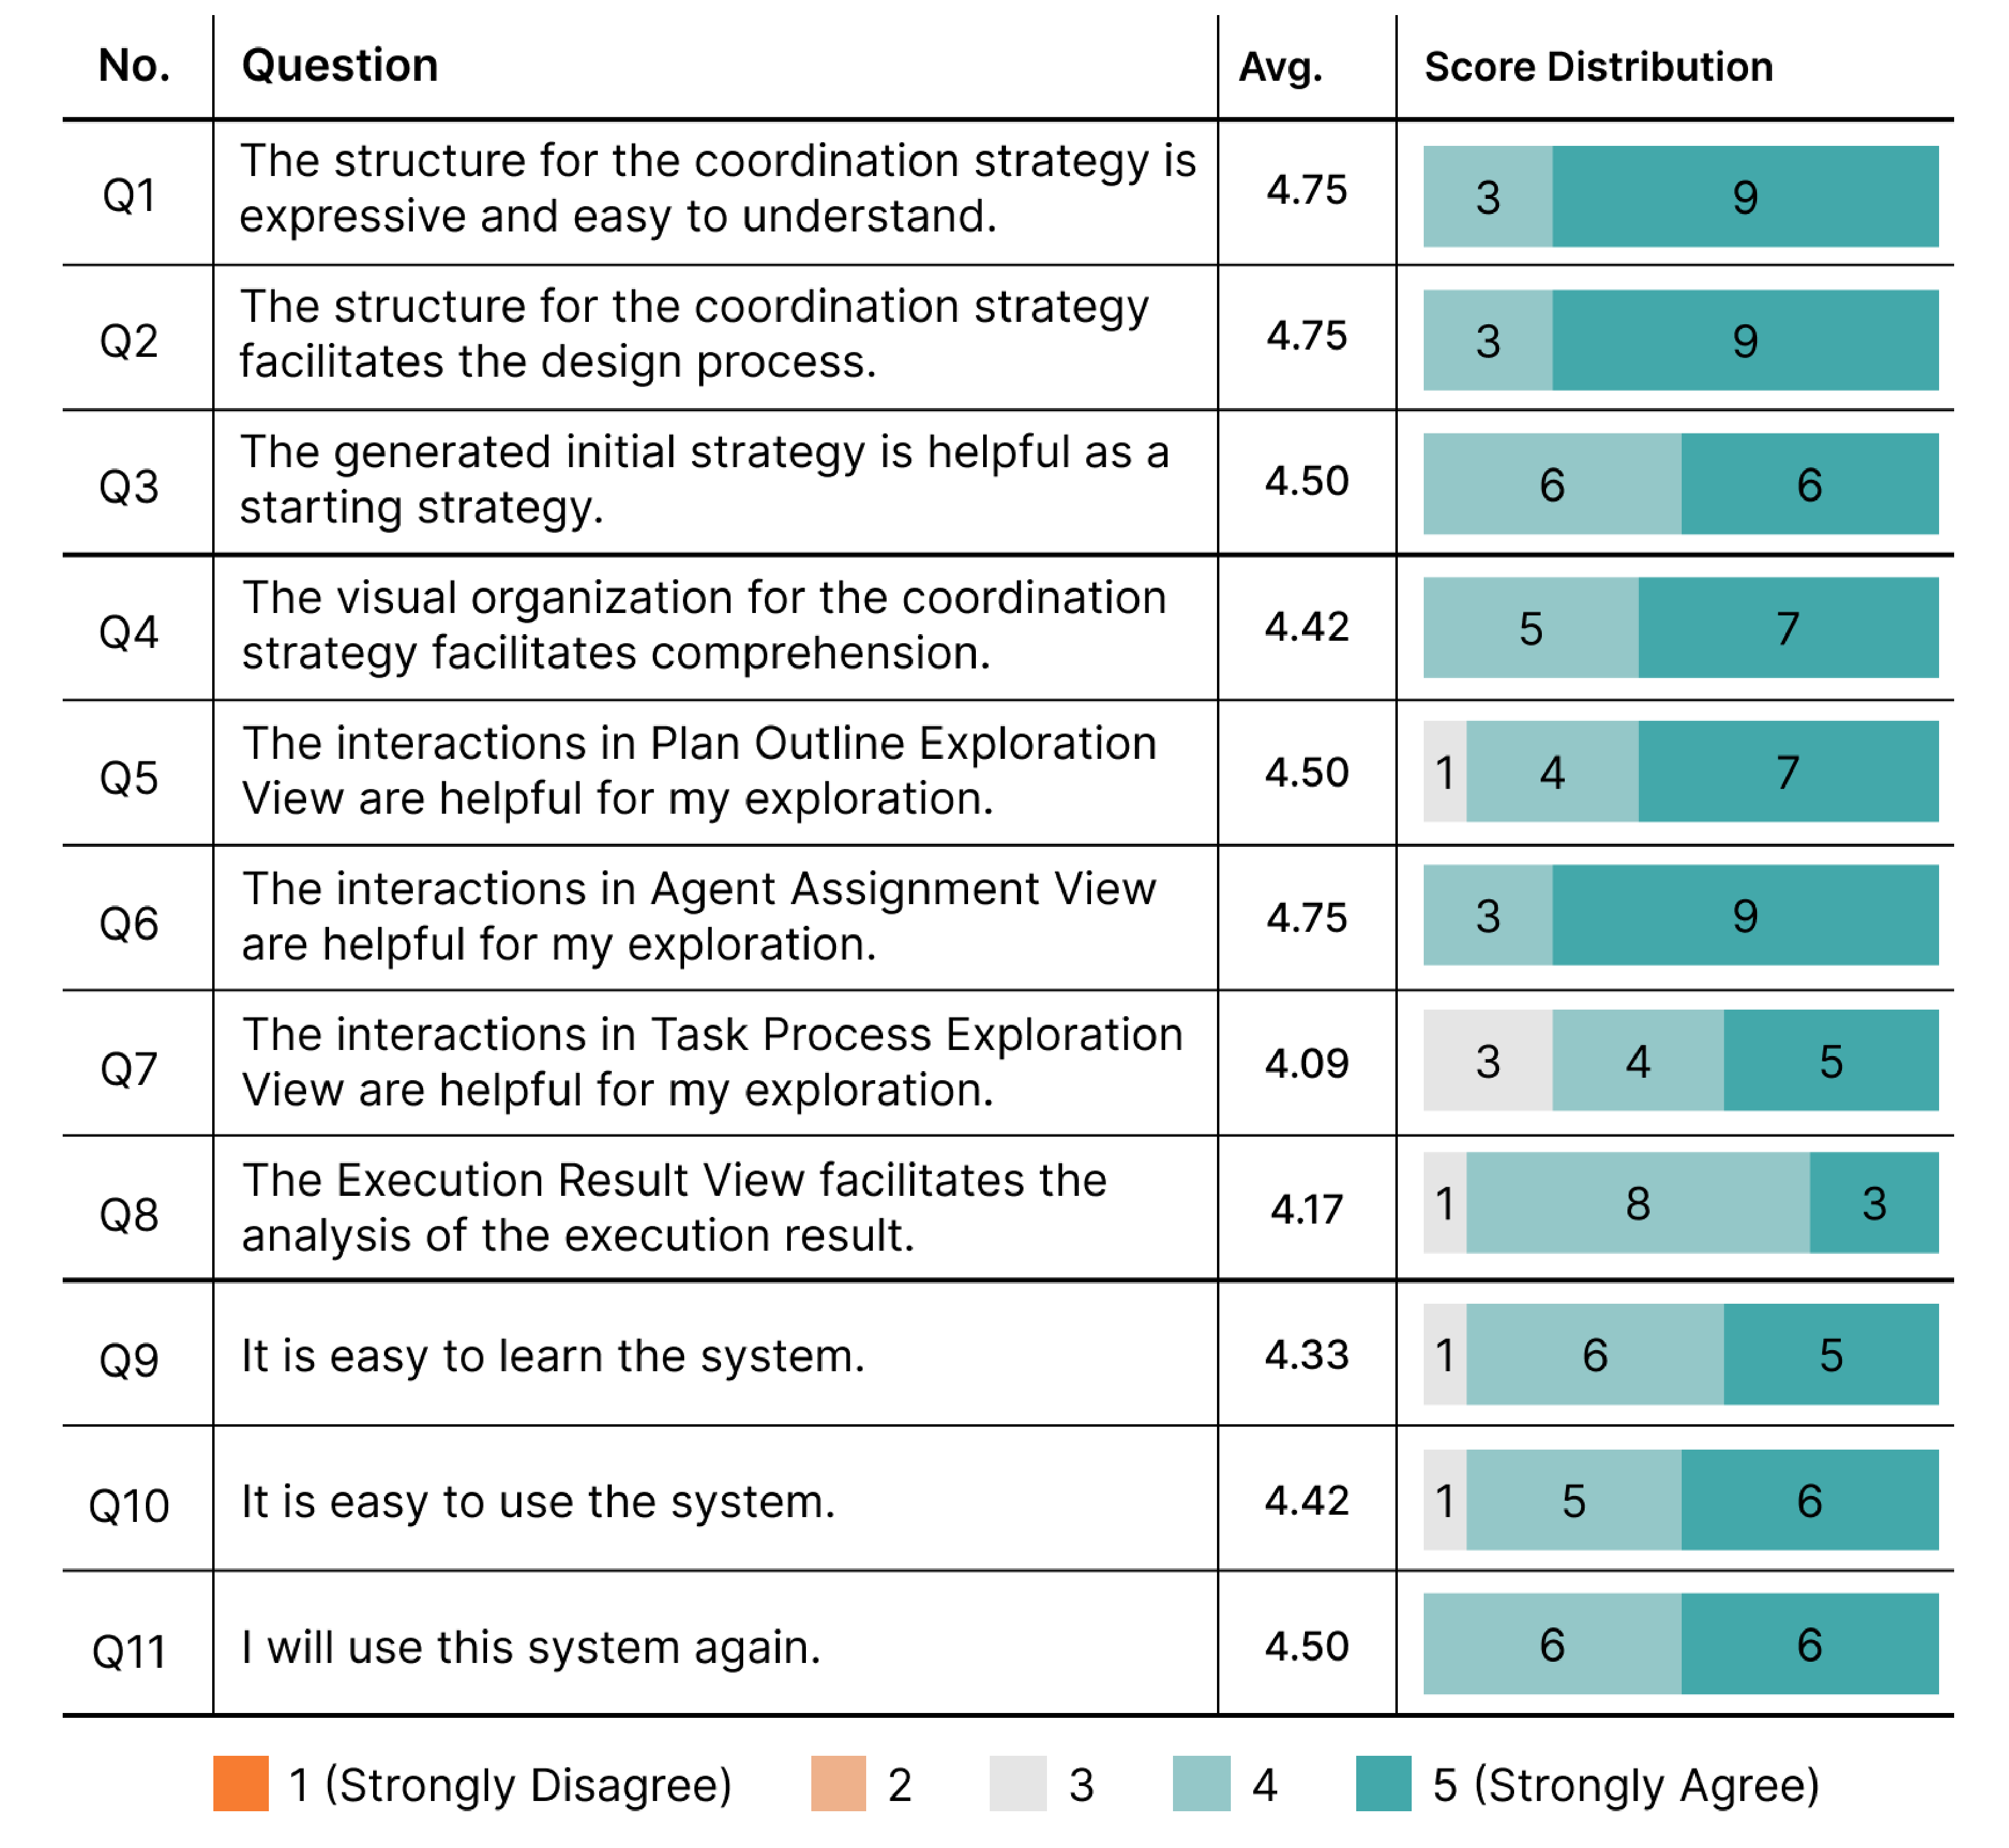
\includegraphics[width=1\linewidth]{figs/evaluation1.pdf}
    \caption{The results of the questionnaire regarding our system’s effectiveness and usability.}
    \label{fig:effectiveness and usability}
\end{figure}
\begin{figure}[!t]
    \centering
    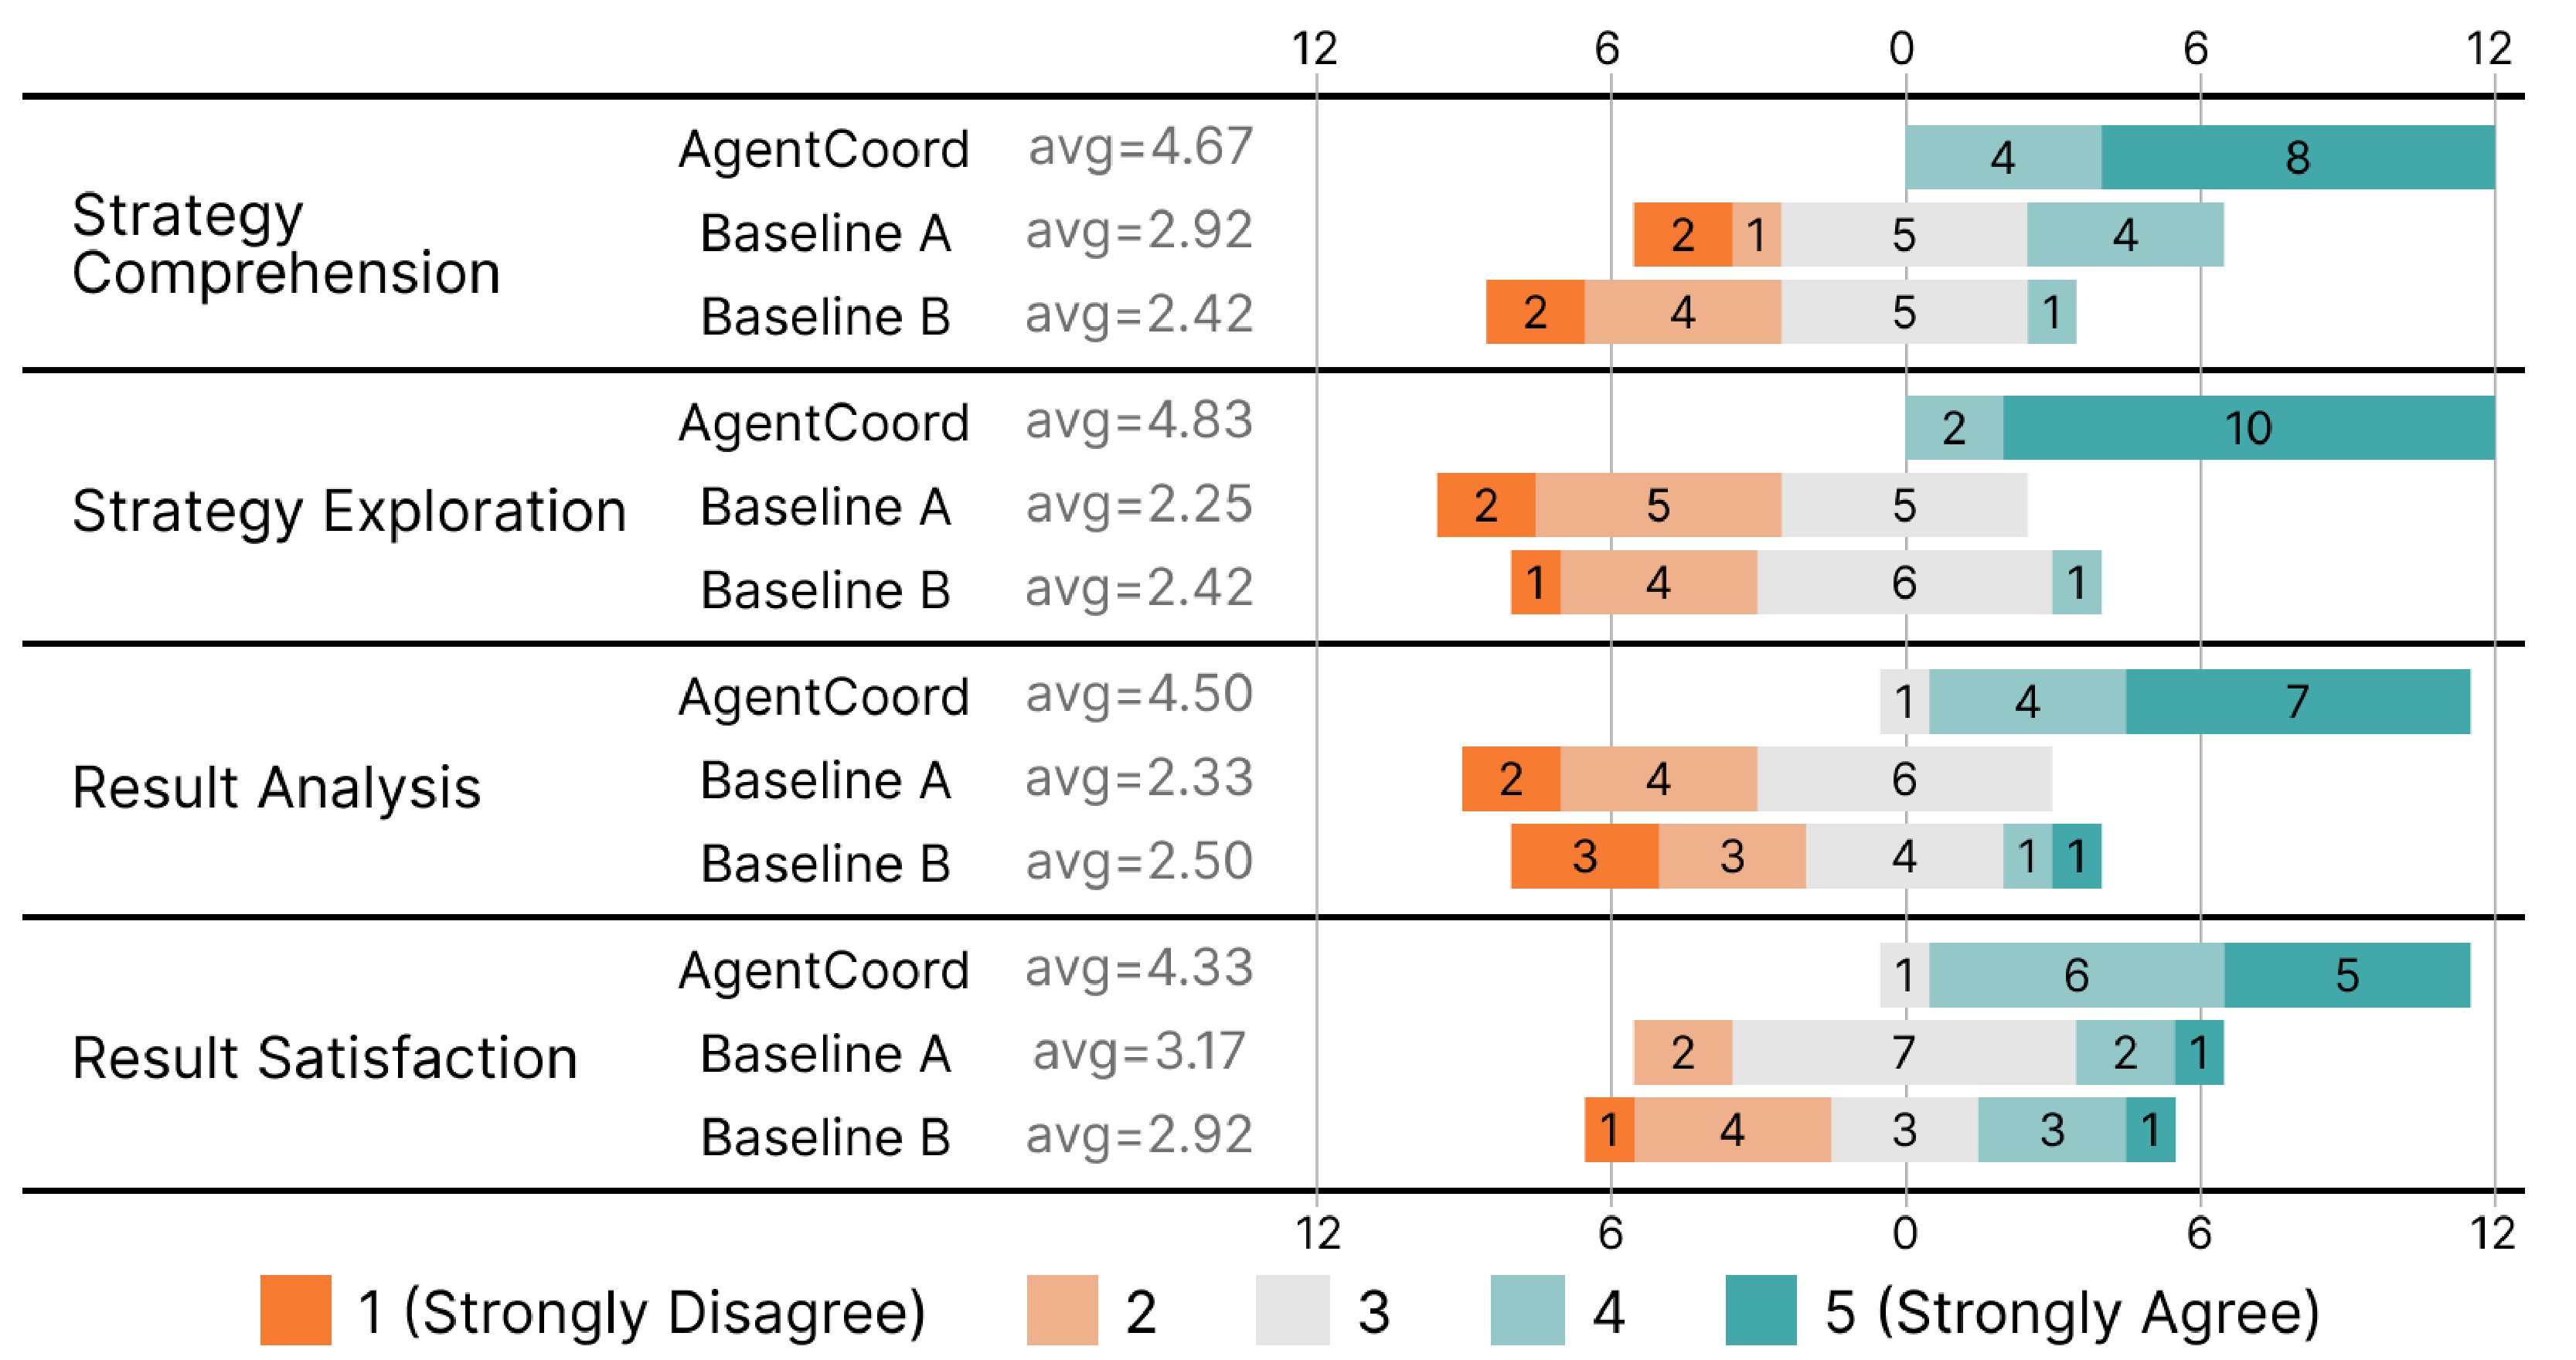
\includegraphics[width=1\linewidth]{figs/evaluation2.pdf}
    \caption{The results of the questionnaire comparing the support for coordination strategy design across the three systems.}
    \label{fig:Coordination Support Comparison}
\vspace{-10pt}
\end{figure}




\subsubsection{Coordination Support Comparison}
To compare our system against two baselines in aiding the design process for coordination strategy, we requested participants to rate three systems across three facets (i.e. strategy comprehension, strategy exploration, and result analysis) of the design process and their satisfaction with the final result. Overall, our system outperforms the baselines for all four aspects. We summarize the user's feedback as follows:

\textbf{Strategy Comprehension}: In Baseline B, the baseline coordination strategy is generated and refined by a planner agent without any structure constraints. Therefore, during the iteration for strategies, ``\textit{the format of strategy could fluctuate frequently, which makes me inconfident}'' (P3). In Baseline A, the strategy is generated with carefully designed prompts that enforce some formats (e.g. divide into steps, and assign agents for each step). However, reading and comparing strategies repented in the pure text still makes users ``\textit{feeling stressed}'' (P11) and ``\textit{less confident for comprehension}'' (P8). In contrast, our system makes sure the coordination strategy has a consistent structure during the whole design process and provides visual organization and enhancement to facilitate comprehension.

\textbf{Strategy Exploration}: In baseline A, no direct support for strategy exploration is provided, users can only use ChatGPT to aid their exploration. However, transferring strategies between interfaces and making manual modifications for format and logic consistency can be ``tedious and error-prone'' (P7). Baseline B allows users to explore alternative strategies by chatting with the planner agent. However, there lack of support for users to flexibly explore different aspects of the strategy on need. Moreover, the quantity of texts can be quickly overwhelming for both the planner agent and users as the process of exploration gets complicated. Our system empowers users with a set of interactions to flexibly explore different aspects of the strategies with the help of LLM and helps visually organize the exploration history.   

\textbf{Result Analysis}: Our system is overall deemed more helpful for execution result analysis. In both baseline A and baseline B, the execution result is directly output to the text terminal. P9 told us that she has to ``sift through the text myself repeatedly to trace the dependencies between execution results and previous operations'' (P9). Instead, in our system, users can easily trace each result back to its important influencing precursors and corresponding coordination strategies.

\textbf{Result Satisfaction}: Compared to Baseline A and Baseline B, users are overall more satisfied with the results of our system. In Baseline B, due to the ambiguity frequently existing in the free-form coordination strategy, the execution process often deviates from the user’s expectations midway and strays further and further away, sometimes even falling into an infinite loop. In Baseline A, thanks to the enforced step-by-step strategy format, there is no infinite loop issue. However, the result usually misses some important parts that should appear according to the coordination strategy (e.g. the main characters decided in character design stages are not shown in the final story). While such problems also exist in the result of our system, users usually can successfully trace the cause by analyzing the result with our system, and quickly adjust the corresponding part of the strategy to fix it.  



 




% “”，‘’,""
% `` \textit{}  ''




